\documentclass[11pt,a4paper]{article}

% ===========================================================================
% Settings
% ===========================================================================
\newcommand{\repourl}{\url{https://github.com/Kyojur0/explainable-dr-grading}}
\newcommand{\reportdate}{October 2026}
\newcommand{\wordcount}{1,929}

% ===========================================================================
% Layout: clean and minimal. Text is black; colour appears only in figures.
% ===========================================================================
\usepackage[a4paper,top=1.8cm,bottom=2.0cm,left=1.9cm,right=1.9cm,footskip=0.9cm]{geometry}
\usepackage[T1]{fontenc}
\usepackage{charter}                 % sturdy, readable text face
\usepackage{tgheros}                 % clean sans for headings and captions
\usepackage[italic]{mathastext}      % maths in the text face, so numbers match
\usepackage{microtype}
\usepackage{xcolor}
\usepackage{graphicx}
\usepackage{float}
\usepackage{booktabs}
\usepackage{colortbl}
\usepackage{url}
\usepackage[font=small,labelfont={bf,sf},labelsep=period,skip=5pt]{caption}
\usepackage{titlesec}
\usepackage{enumitem}
\usepackage{needspace}

\linespread{1.04}
\definecolor{muted}{HTML}{5A5A5A}
\definecolor{accent}{HTML}{2B6CB0}
\definecolor{tint}{HTML}{EAF1F8}
\titleformat{\section}{\normalfont\sffamily\large\bfseries}{\thesection}{0.7em}{}
\titleformat{\subsection}{\normalfont\sffamily\normalsize\bfseries}{\thesubsection}{0.7em}{}
\titlespacing*{\section}{0pt}{1.3ex}{0.5ex}
\titlespacing*{\subsection}{0pt}{0.9ex}{0.25ex}
\setlist{nosep,leftmargin=1.3em,topsep=0.15em}
\setlength{\parindent}{0pt}
\setlength{\parskip}{0.45em}
\renewcommand{\arraystretch}{1.22}
\setlength{\heavyrulewidth}{0.7pt}
\setlength{\lightrulewidth}{0.4pt}
\setlength{\aboverulesep}{0pt}
\setlength{\belowrulesep}{0pt}
\newcommand{\header}{\rowcolor{tint}}
\setlength{\textfloatsep}{10pt plus 2pt minus 2pt}
\setlength{\floatsep}{8pt plus 2pt minus 2pt}
\setlength{\intextsep}{8pt plus 2pt minus 2pt}
\graphicspath{{figures/}}
\urlstyle{same}

\begin{document}

% ===========================================================================
{\sffamily
{\LARGE\bfseries Explainable deep learning for diabetic retinopathy grading}\\[0.3em]
{\large Colour fundus photographs from MMRDR}\\[0.7em]
{\small Haroon Ayaz \quad\textbullet\quad Practical assessment, KTP Associate, ref.\ 1443-26 \quad\textbullet\quad \reportdate}\\[0.2em]
{\small\color{muted} Code: \repourl \quad\textbullet\quad Word count \wordcount, excluding references\\ Research prototype, not a clinically validated device}\par}
\vspace{0.5em}{\color{muted}\rule{\linewidth}{0.4pt}}
\vspace{0.3em}

% ===========================================================================
\section{Introduction and objectives}

Diabetic retinopathy (DR) grading decides who is referred to an eye specialist. An optometrist using a grading aid needs the grade, how far to trust it, and what in the image drove it. I trained a five-grade classifier (ICDR grades 0 to 4 \cite{wilkinson2003}) on MMRDR colour fundus photographs \cite{mmrdr2026}, tested it once, measured its reliability, and tested whether its Grad-CAM maps reflect the model. Referable DR here means grade 2 or above, the usual research definition \cite{gulshan2016}; NHS screening also refers maculopathy \cite{desp}, which this model does not assess.

% ===========================================================================
\section{Data and methods}

\begin{figure}[ht]
\centering
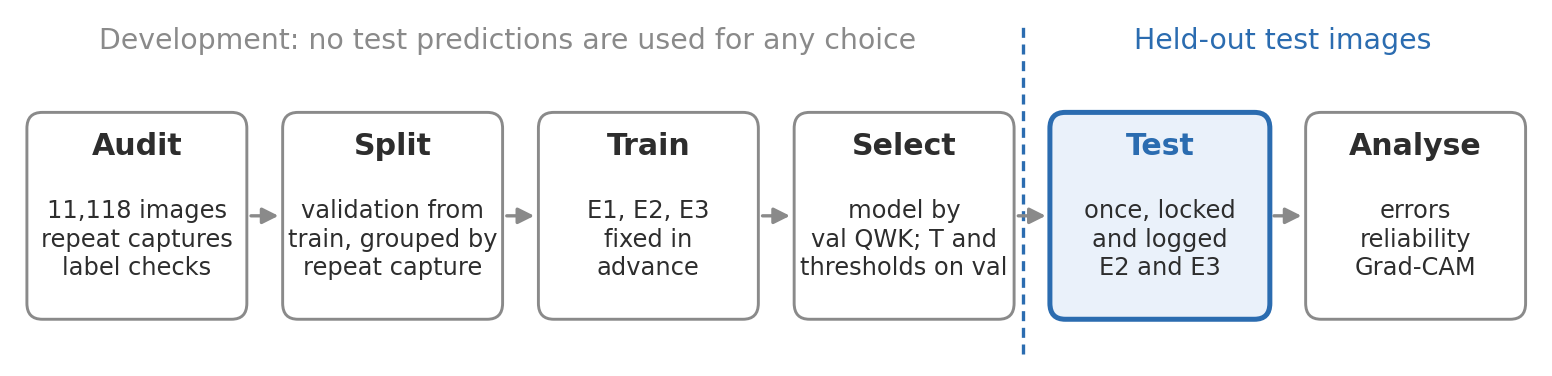
\includegraphics[width=\linewidth]{overview.png}
\caption{The pipeline. Every choice was made before any test prediction existed.}
\label{fig:overview}
\end{figure}

\subsection{Data audit}
MMRDR has 11,118 photographs (8,893 train, 2,225 test) from the OIA-DDR dataset \cite{ddr2019}, each with a grade and seven lesion flags that record presence, not location. 59\% are grade 0, and the largest training class is 10.4 times the smallest. The source has no patient identifiers, so the official split is by image \cite{mmrdr2026}. The audit read every image and label but used no model. All images were readable, at 1,857 resolutions. It found three issues:
\begin{itemize}
  \item \textbf{Repeat captures.} Perceptual hashing matched different eyes, so I built a vessel-pattern signature instead. It found 148 groups of repeat captures (one later judged a false match by eye). 50 test images have a copy in train, and 4 groups disagree on grade.
  \item \textbf{Grade 1 labels.} Grade 1 means microaneurysms only, yet 116 of the 259 grade 1 test images carry another lesion flag.
  \item \textbf{Camera background.} 63 test images have a grey background; 63\% of them are referable, against 29\% overall.
\end{itemize}

\subsection{Split and preprocessing}
Validation (1,268 images) was taken from the training set in whole repeat-capture groups, stratified by grade (shares differ by at most 0.09 percentage points). The test set was left as published. Images were cropped to the fundus, padded square, resized to 512 px and blacked out outside the inscribed circle, which removes the background. Augmentation used rotation, flips, cropping, brightness, contrast and gamma, but no hue change, because colour carries clinical meaning.

\subsection{Models and training}
Three runs were declared before training: E1, ResNet-18 \cite{he2016} at 384 px with class-weighted loss, as a simple baseline; E2, EfficientNet-B0 \cite{tan2019} at 512 px; and E3, E2 with class weights $(N/n_c)^{1/2}$. EfficientNet-B0 is accurate for its size, so it can train at 512 px, where small lesions stay visible, and its pooling and linear head make Grad-CAM exact (Section~\ref{sec:xai}). All start from ImageNet weights in \texttt{timm} \cite{timm}. Hyperparameters were common transfer-learning defaults, fixed in advance and not tuned: AdamW (learning rate $3\times10^{-4}$, weight decay $10^{-4}$), batch size 16, cosine decay, and up to 20 epochs with early stopping on validation quadratic weighted kappa (QWK) \cite{cohen1968}. The run with the best validation QWK was selected, because QWK penalises a grade 4 called 0 far more than a near miss. The referable operating point was set separately, by threshold (Section~\ref{sec:rel}). A majority-class baseline (M0) sets the floor.

\subsection{Evaluation protocol}
No model, hyperparameter, temperature or threshold was chosen using test labels or predictions, and every extra run finished before testing. Two models were declared for testing: E2 (selected) and E3 (comparison). Each was predicted on test once, under a lock that refuses a second run, and every read of test images was logged. Before testing, a separate AI agent reviewed the pipeline and its findings were fixed. Intervals are 95\% bootstraps (1,000 resamples).

% ===========================================================================
\section{Results}

\begin{table}[ht]
\centering\small
\caption{Validation ($n = 1{,}268$), from predictions saved during training. The rule selects E2.}
\label{tab:val}
\begin{tabular}{lcccc}
\toprule
\header Run & Accuracy & Macro-F1 & QWK & Referable sensitivity \\
\midrule
E1\enspace ResNet-18, 384 px, weighted & 0.827 & 0.730 & 0.918 & 0.846 \\
E2\enspace EfficientNet-B0, 512 px & 0.853 & 0.754 & \textbf{0.929} & 0.843 \\
E3\enspace EfficientNet-B0, 512 px, weighted & 0.843 & 0.757 & 0.924 & 0.919 \\
\bottomrule
\end{tabular}
\end{table}

Three runs of the E2 recipe (seed 42, seed 43, and seed 42 on other hardware) gave validation QWK from 0.926 to 0.932, so gaps of a few thousandths are noise. Neither 384 px nor test-time augmentation improved E2.

\begin{table}[ht]
\centering\small
\caption{Test results ($n = 2{,}225$) with 95\% intervals. M0 always predicts grade 0.}
\label{tab:test}
\begin{tabular}{lccc}
\toprule
\header & M0 & E2 (selected) & E3 (weighted) \\
\midrule
Accuracy & 0.595 & 0.830\enspace(0.813--0.845) & 0.822\enspace(0.806--0.837) \\
Macro-F1 & 0.149 & 0.725\enspace(0.697--0.751) & 0.709\enspace(0.683--0.732) \\
QWK & 0.000 & 0.907\enspace(0.894--0.920) & 0.907\enspace(0.893--0.919) \\
Referable sensitivity & 0.000 & 0.793\enspace(0.762--0.823) & 0.865\enspace(0.838--0.891) \\
Referable specificity & 1.000 & 0.949 & 0.927 \\
Referable AUROC & -- & 0.967 & 0.968 \\
QWK without 50 copies & -- & 0.906 & 0.906 \\
\bottomrule
\end{tabular}
\end{table}

\begin{figure}[ht]
\centering
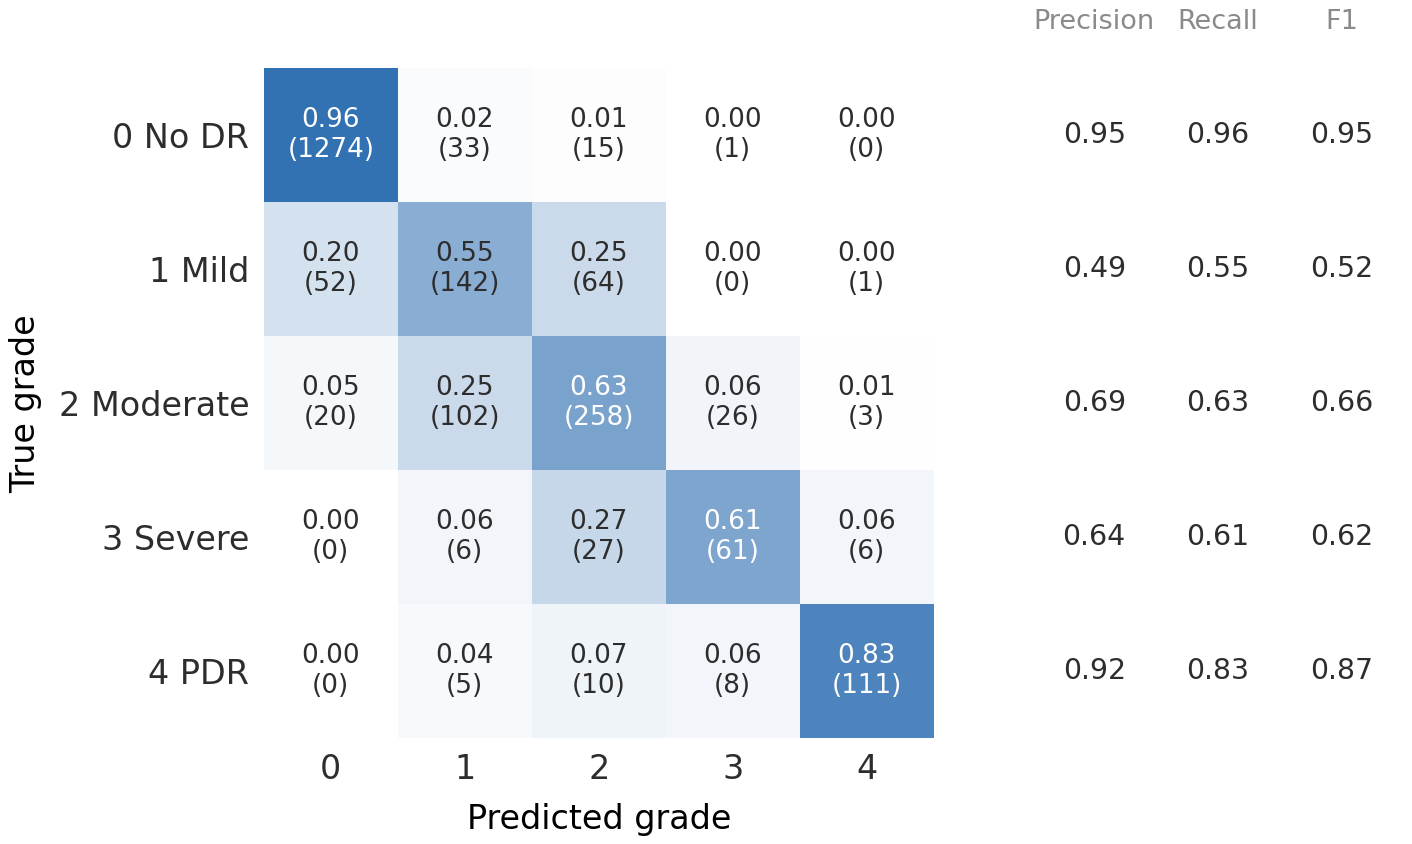
\includegraphics[width=0.8\linewidth]{confusion.png}
\caption{E2 on test, by true grade, with per-class precision, recall and F1.}
\label{fig:cm}
\end{figure}

Test QWK was 0.022 below validation for E2 and 0.018 for E3; selecting on validation makes it optimistic, so test is the figure I report. Removing the 50 copied images changed QWK by 0.001, so the detected copies do not explain the result, though overlap between eyes of one patient cannot be measured.

\textbf{Error analysis.} Only 2.7\% of predictions were two or more grades out (Figure~\ref{fig:cm}). The costly direction is underestimation: 133 of 643 referable images (20.7\%) were graded 0 or 1, 113 of them as grade 1, and 15 of 134 proliferative images were graded 2 or below. Grade 1 is the weakest class (F1 0.52), in line with its inconsistent labels. E3 gave the same QWK with higher referable sensitivity (0.865) and grade 3 recall (0.81 against 0.61), at lower specificity. Accuracy on the grey-background images was 0.65, which their grade mix alone predicts.

% ===========================================================================
\section{Reliability}
\label{sec:rel}

All settings were fitted on validation and applied unchanged to test.
\begin{itemize}
  \item \textbf{Calibration.} E2 was overconfident. Temperature scaling \cite{guo2017} ($T = 2.26$) cut the expected calibration error on test from 0.103 to 0.023, without changing any grade.
  \item \textbf{Referral.} Referring the 20\% of cases with the lowest calibrated confidence caught 79 of the 133 referable misses on test (59\%). A second rule, set on validation to keep the miss rate among retained cases at 5\%, referred 36\% on test, but that miss rate was 7.9\%, so the target did not hold.
  \item \textbf{Operating point.} The referable score is the calibrated probability of grades 2 to 4. A threshold declared before testing, set to match E3's validation sensitivity, gave E2 a test sensitivity of 0.885 at specificity 0.926, against 0.865 at 0.927 for E3. Selecting by QWK therefore cost no referable sensitivity.
\end{itemize}

\begin{figure}[ht]
\centering
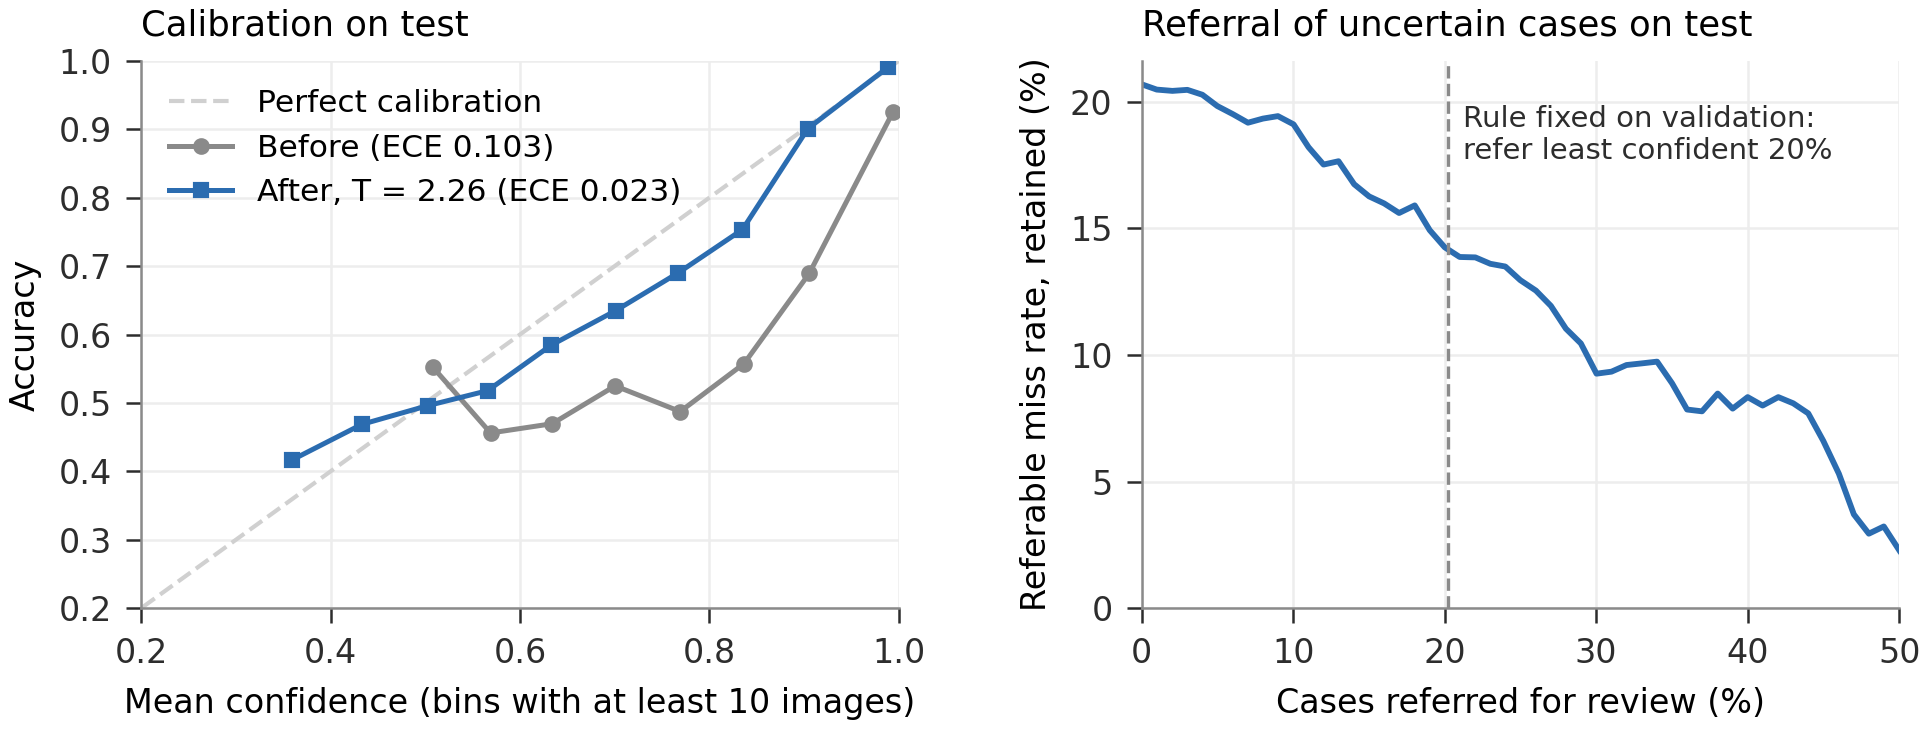
\includegraphics[width=\linewidth]{reliability.png}
\caption{E2 on test. Left: calibration. Right: referable miss rate among cases kept, as more uncertain cases are referred.}
\label{fig:rel}
\end{figure}

% ===========================================================================
\section{Explainability}
\label{sec:xai}

I used Grad-CAM \cite{selvaraju2017} on EfficientNet-B0's final feature map. Because this map feeds average pooling and a linear layer, Grad-CAM there equals class activation mapping \cite{zhou2016} up to scale, which a unit test checks. Maps are $16 \times 16$ cells, enough to locate regions but not single microaneurysms. Three checks were run on validation:
\begin{itemize}
  \item \emph{Model randomisation} \cite{adebayo2018} (50 images). Re-initialising the classifier dropped the rank correlation with the trained map to $-0.20$, and randomising all layers left it at 0.07, near the 0.10 of unrelated images. This shows the maps depend on the classifier, which is expected at this layer.
  \item \emph{Deletion} (200 images, Figure~\ref{fig:del}). Blurring the most salient 5\% of fundus pixels lowered the predicted-class probability by 0.17, against 0.06 for the same mask rotated elsewhere and 0.01 for random pixels. For predicted grades 1 to 3 the salient patch beat the rotated one by 0.26 to 0.46; for grade 0 they were equal.
  \item \emph{Shortcuts} (1,268 images). The fundus edge got less than its share of attention, but the brightest region, a proxy for the optic disc, got 3.7 times its share.
\end{itemize}

\begin{figure}[H]
\centering
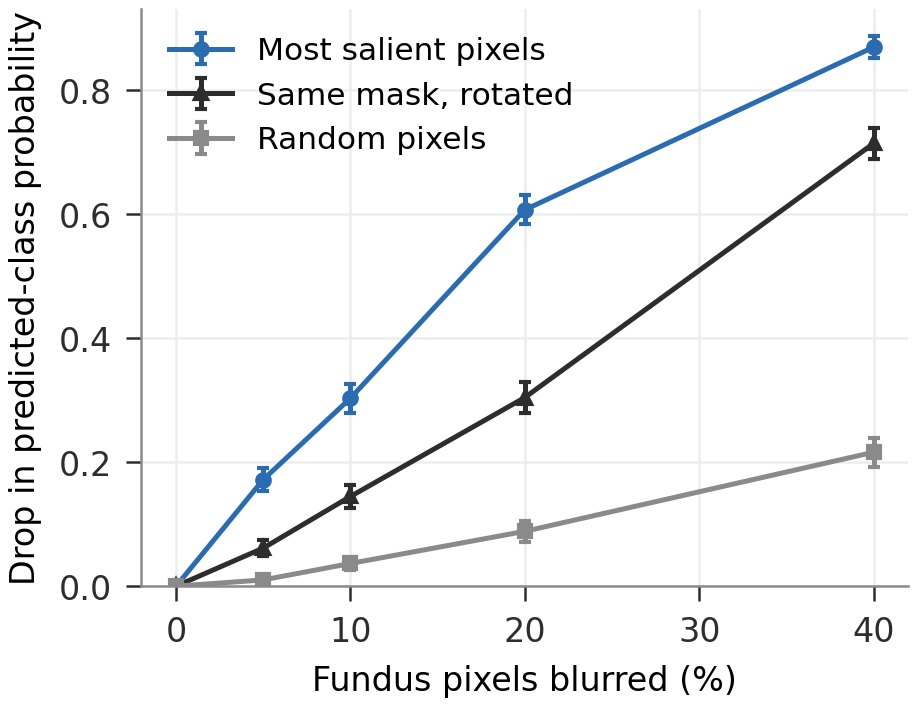
\includegraphics[width=0.42\linewidth]{deletion.png}
\caption{Deletion test: mean drop in predicted-class probability, with standard errors.}
\label{fig:del}
\end{figure}

\begin{figure}[t]
\centering
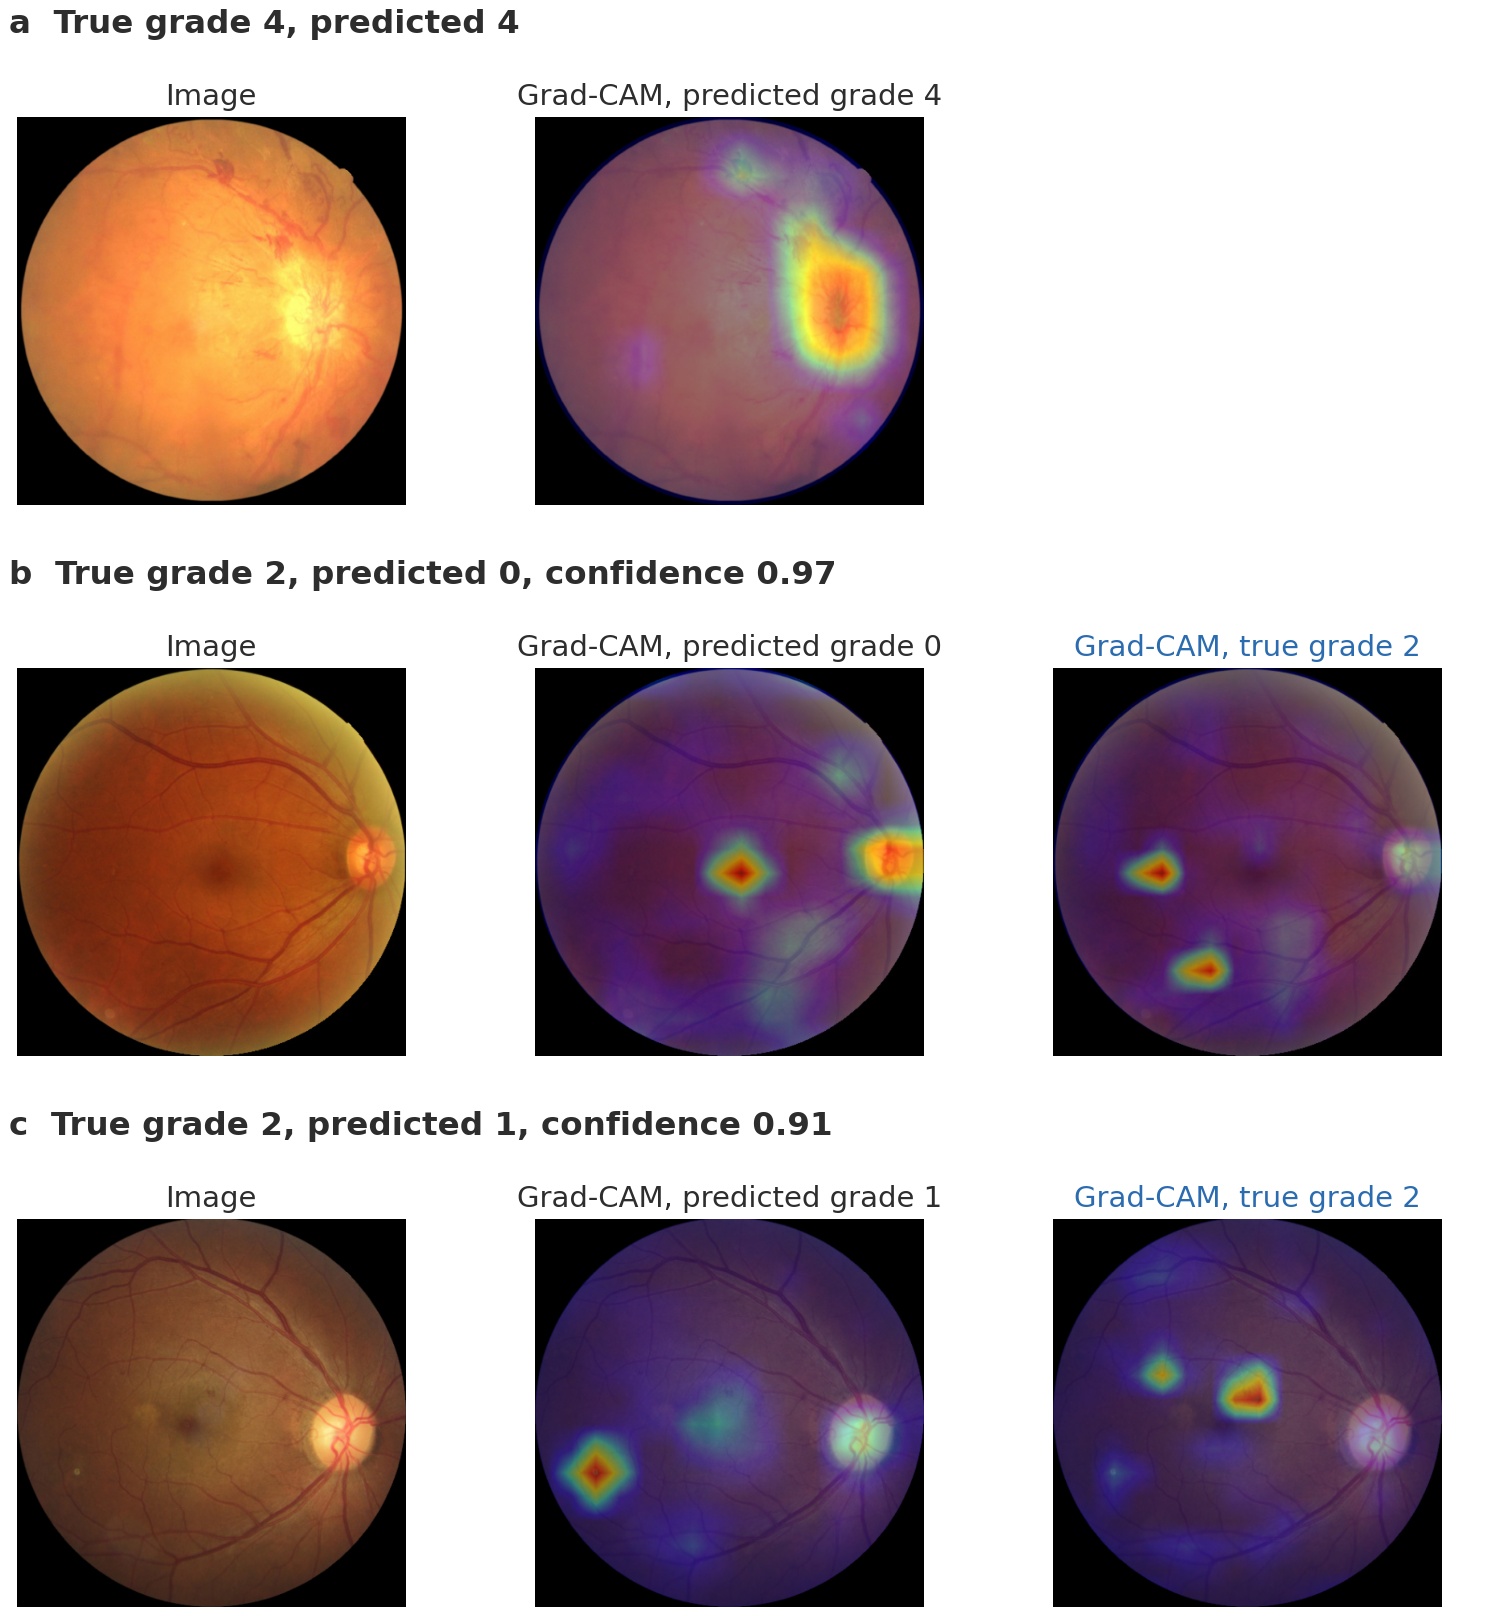
\includegraphics[width=0.86\linewidth]{cam_cases.png}
\caption{Grad-CAM on test images. (a) Proliferative DR graded correctly. (b, c) Moderate DR graded 0 and 1 with high confidence; the 20\% rule would refer neither.}
\label{fig:cam}
\end{figure}

\textbf{Clinical reading.} In Figure~\ref{fig:cam}a the map lies on the optic disc. That fits new vessels at the disc, but also the disc attention seen across all images, and the map cannot tell the two apart. Grad-CAM explains the predicted grade, so for a referable eye graded 0 it shows what raised the grade 0 score. In 6 of the 12 misses I reviewed by eye, that was the fovea or disc, while the map for the true grade often pointed elsewhere (Figure~\ref{fig:cam}b, c). All 12 were selected as the most confident errors and none would have been referred: a confident grade with a plausible map can still be wrong. Lesion flags have no locations, so overlap cannot be measured; with grade held fixed, none of 39 lesion comparisons survived correction for multiple testing \cite{benjamini1995}. Deletion shows the maps reflect the model, not lesions, and blurred patches are unlike training images \cite{hooker2019}.

An optometrist would see the grade, calibrated confidence and review flag first, with the map as a supporting view and a map for the referable grade when the grade is 0 or 1. The decision stays with the clinician.

% ===========================================================================
\section{Anticipated challenge and proposed strategy}

The advert describes ``scaling explainable AI-enabled triage within a clinical retail setting''. I think the hardest part is not the model but keeping its output safe afterwards: on the right record, with its uncertainty, with the optometrist's action recorded, and still valid as cameras change across more than 500 practices.

Results are fragile even within one dataset: here the 5\% target became 7.9\% on test, and confident errors escaped referral. In the HERMES trial, the AI read OCT scans and could process images from only 52\% of participants \cite{sharma2025}; seven DR systems varied in real-world use \cite{lee2021}; and clinicians over-trust automated advice \cite{goddard2012}. My EPR work shows another risk. In a build I work on, laboratory messages lost the link between blood-culture bottles and their comments. The results were right; the integration broke them. An AI grade attached to the wrong image would fail the same way.

\needspace{5\baselineskip}\textbf{Strategy.}
\begin{enumerate}
  \item Agree with optometrists the decision, the reference standard (hospital outcome), the acceptable miss rate and the mapping to NHS grading, and fix thresholds before testing.
  \item Define the record first: image and episode identifiers, model version, confidence and review flag, with the optometrist's decision and any override beside them.
  \item Validate on Boots data by device, practice, image quality and patient group, then run the model silently in a few practices.
  \item Pilot the assisted version, with usability tests that include planted wrong outputs.
  \item Re-run automated end-to-end tests after every change. I built such a suite in my current role: one parameterised flow designed to cover 457 imaging codes. Changes go through DCB0129 and DCB0160 clinical risk management \cite{dcb0129,dcb0160} and a DPIA.
\end{enumerate}
\textbf{Evaluation:} urgent-referral sensitivity no worse than current practice, fewer false-positive referrals, calibration by device, override rates and reasons, and no mismatched records. \textbf{Risks:} noisy reference labels, verification bias (only referred patients get a hospital outcome), alert fatigue and device changes.

% ===========================================================================
\section{Limitations and conclusions}

The split is by image, so one person's eyes may fall on both sides. All images come from one source, with no camera or demographic metadata and no external validation. Bootstrap intervals treat images as independent, and calibration rests on 1,268 validation images.

EfficientNet-B0 reached test QWK 0.907 and accuracy 0.830, against 0.595 for always predicting no DR. Its main weakness is underestimating referable disease. Calibration and referral catch most of those cases, but confident errors get through, and Grad-CAM cannot show what the model missed. Next steps are patient-level splits, external validation across cameras, and measuring map overlap on the DDR images that have lesion masks \cite{ddr2019}. This is a research prototype, not a clinical tool.

\textbf{Tools and resources.} \texttt{timm} weights \texttt{efficientnet\_b0.ra\_in1k} and \texttt{resnet18.a1\_in1k} \cite{timm}; PyTorch, torchvision, NumPy, pandas, scikit-learn, SciPy, Pillow and matplotlib. Developed with the help of AI coding tools. Every number can be recomputed from outputs in the repository.

% ===========================================================================
\begin{thebibliography}{99}
\small
\setlength{\itemsep}{1pt}
\bibitem{wilkinson2003} C.~P. Wilkinson et al., ``Proposed international clinical diabetic retinopathy and diabetic macular edema disease severity scales,'' \emph{Ophthalmology}, vol.~110, no.~9, pp.~1677--1682, 2003.
\bibitem{mmrdr2026} Z.~Tang et al., ``A multimodal retinal image dataset for diabetic retinopathy detection using foundation models,'' \emph{Scientific Data}, vol.~13, art.~639, 2026.
\bibitem{gulshan2016} V.~Gulshan et al., ``Development and validation of a deep learning algorithm for detection of diabetic retinopathy in retinal fundus photographs,'' \emph{JAMA}, vol.~316, no.~22, pp.~2402--2410, 2016.
\bibitem{desp} Public Health England, ``NHS Diabetic Eye Screening Programme: grading definitions for referable disease,'' GOV.UK. Accessed: Oct.\ 2026.
\bibitem{ddr2019} T.~Li, Y.~Gao, K.~Wang, S.~Guo, H.~Liu and H.~Kang, ``Diagnostic assessment of deep learning algorithms for diabetic retinopathy screening,'' \emph{Information Sciences}, vol.~501, pp.~511--522, 2019.
\bibitem{he2016} K.~He, X.~Zhang, S.~Ren and J.~Sun, ``Deep residual learning for image recognition,'' in \emph{Proc.\ CVPR}, 2016, pp.~770--778.
\bibitem{tan2019} M.~Tan and Q.~V. Le, ``EfficientNet: Rethinking model scaling for convolutional neural networks,'' in \emph{Proc.\ ICML}, 2019, pp.~6105--6114.
\bibitem{timm} R.~Wightman, ``PyTorch Image Models,'' 2019. [Online]. Available: \url{https://github.com/huggingface/pytorch-image-models}
\bibitem{cohen1968} J.~Cohen, ``Weighted kappa: Nominal scale agreement with provision for scaled disagreement or partial credit,'' \emph{Psychological Bulletin}, vol.~70, no.~4, pp.~213--220, 1968.
\bibitem{guo2017} C.~Guo, G.~Pleiss, Y.~Sun and K.~Q. Weinberger, ``On calibration of modern neural networks,'' in \emph{Proc.\ ICML}, 2017, pp.~1321--1330.
\bibitem{selvaraju2017} R.~R. Selvaraju et al., ``Grad-CAM: Visual explanations from deep networks via gradient-based localization,'' in \emph{Proc.\ ICCV}, 2017, pp.~618--626.
\bibitem{zhou2016} B.~Zhou, A.~Khosla, A.~Lapedriza, A.~Oliva and A.~Torralba, ``Learning deep features for discriminative localization,'' in \emph{Proc.\ CVPR}, 2016, pp.~2921--2929.
\bibitem{adebayo2018} J.~Adebayo et al., ``Sanity checks for saliency maps,'' in \emph{Advances in Neural Information Processing Systems}, 2018.
\bibitem{benjamini1995} Y.~Benjamini and Y.~Hochberg, ``Controlling the false discovery rate: A practical and powerful approach to multiple testing,'' \emph{J.\ R.\ Stat.\ Soc.\ B}, vol.~57, no.~1, pp.~289--300, 1995.
\bibitem{hooker2019} S.~Hooker, D.~Erhan, P.-J. Kindermans and B.~Kim, ``A benchmark for interpretability methods in deep neural networks,'' in \emph{Advances in Neural Information Processing Systems}, 2019.
\bibitem{sharma2025} A.~Sharma et al., ``Teleophthalmology versus standard of care for community optometry referrals of retinal disease (HERMES): a cluster randomised controlled trial with linked prospective diagnostic accuracy assessment of artificial intelligence support,'' \emph{The Lancet Primary Care}, vol.~1, no.~4, art.~100041, 2025.
\bibitem{lee2021} A.~Y. Lee et al., ``Multicenter, head-to-head, real-world validation study of seven automated artificial intelligence diabetic retinopathy screening systems,'' \emph{Diabetes Care}, vol.~44, no.~5, pp.~1168--1175, 2021.
\bibitem{goddard2012} K.~Goddard, A.~Roudsari and J.~C. Wyatt, ``Automation bias: A systematic review of frequency, effect mediators, and mitigators,'' \emph{J.\ Am.\ Med.\ Inform.\ Assoc.}, vol.~19, no.~1, pp.~121--127, 2012.
\bibitem{dcb0129} NHS Digital, ``DCB0129: Clinical risk management: its application in the manufacture of health IT systems,'' 2018.
\bibitem{dcb0160} NHS Digital, ``DCB0160: Clinical risk management: its application in the deployment and use of health IT systems,'' 2018.
\end{thebibliography}

\end{document}
